\subsubsection{Существующая информационная система и её недостатки}

%% \begin{figure}[h]
\center{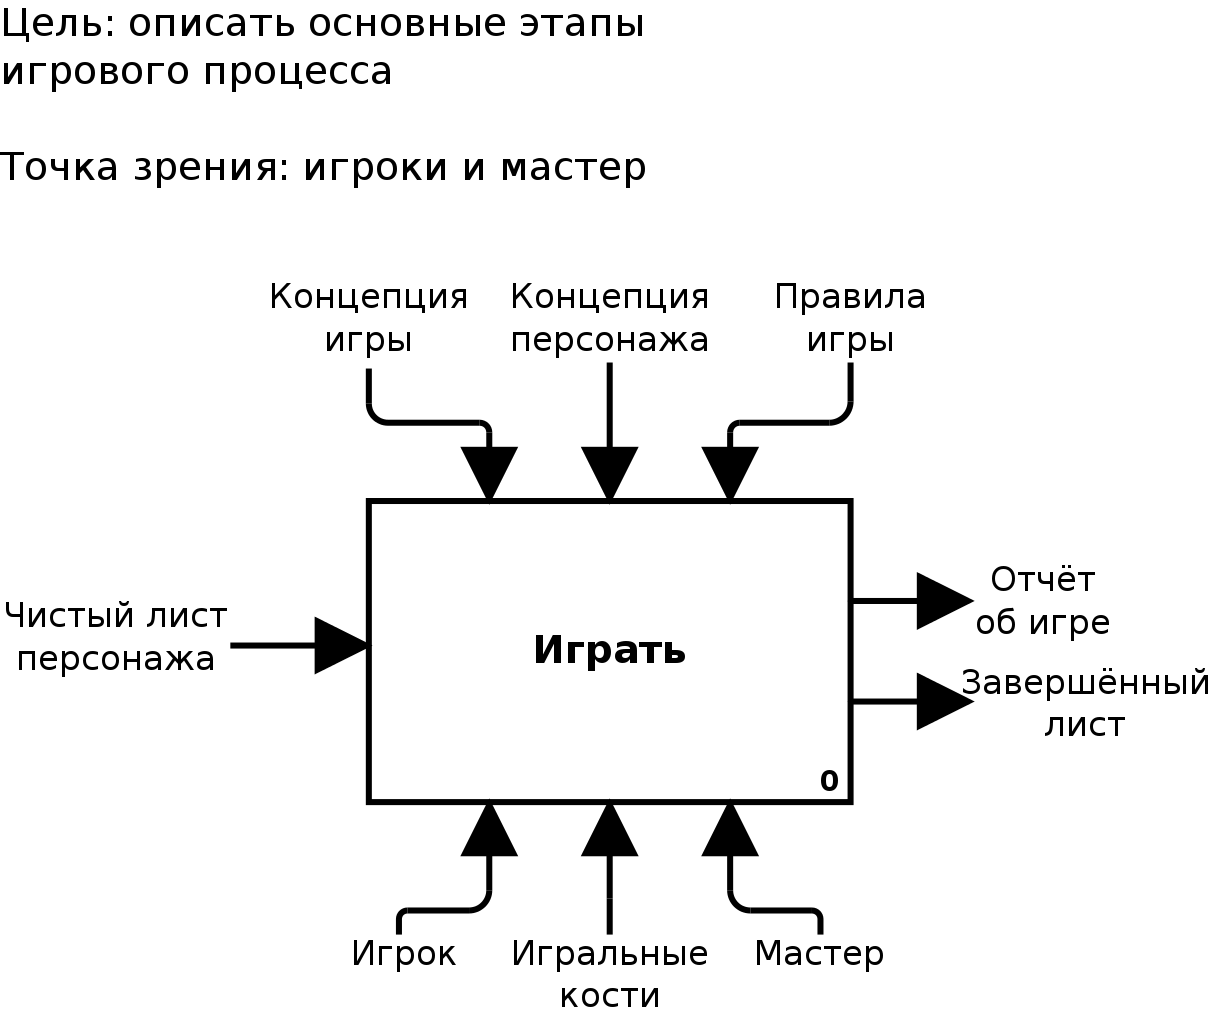
\includegraphics[width=1\linewidth]{images/current_idef/Context.png}}
\caption{Контекстная диаграмма исходной информационной системы}
\label{ris:current_context_diagram}
\end{figure}

\begin{figure}[h]
\center{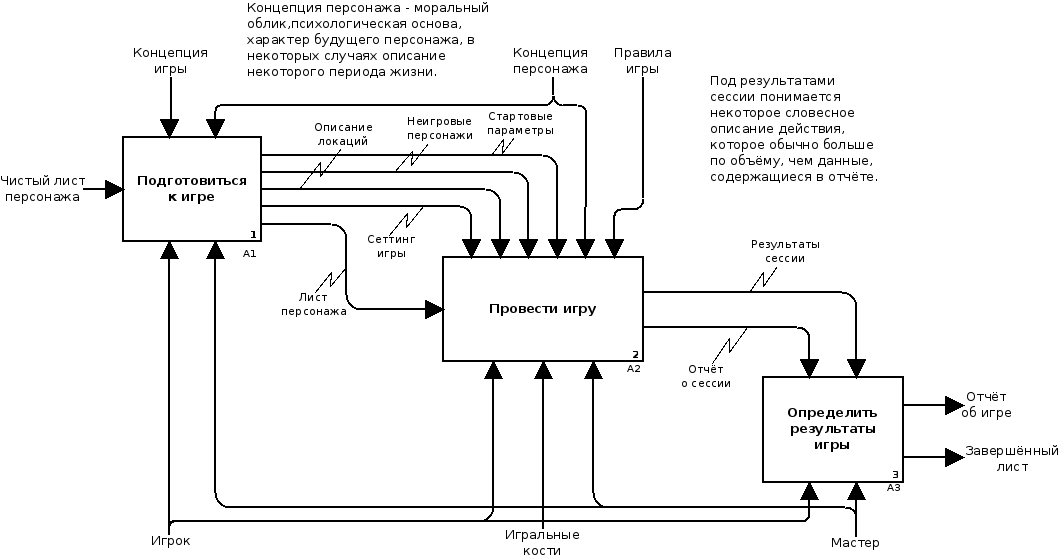
\includegraphics[width=1\linewidth]{images/current_idef/A0.png}}
\caption{Диаграмма A0 исходной информационной системы: описание процесса <<Играть>>}
\label{ris:current_a0_diagram}
\end{figure}

\begin{figure}[h]
\center{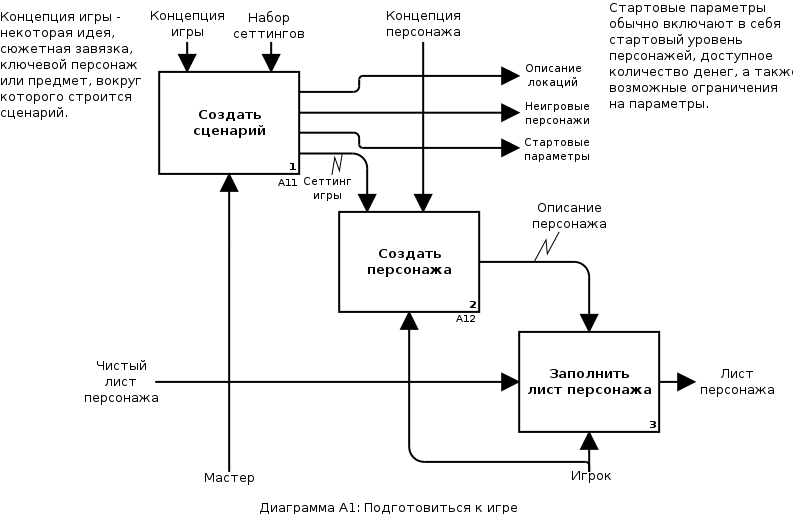
\includegraphics[width=1\linewidth]{images/current_idef/A1.png}}
\caption{Диаграмма A1 исходной информационной системы: описание процесса <<Подготовиться к игре>>}
\label{ris:current_a1_diagram}
\end{figure}

\begin{figure}[h]
\center{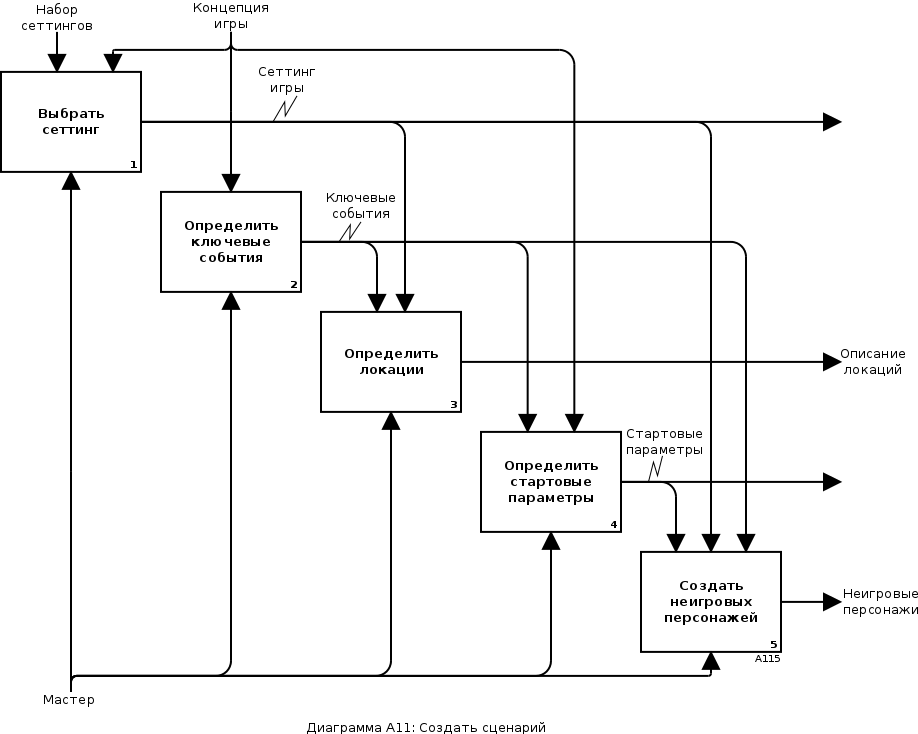
\includegraphics[width=1\linewidth]{images/current_idef/A11.png}}
\caption{Диаграмма A11 исходной информационной системы: описание процесса <<Создать сценарий>>}
\label{ris:current_a11_diagram}
\end{figure}

\begin{figure}[h]
\center{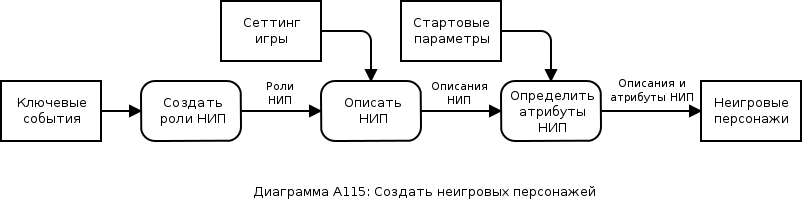
\includegraphics[width=1\linewidth]{images/current_idef/A115.png}}
\caption{Диаграмма A115 исходной информационной системы: описание процесса <<Создать неигровых персонажей>>}
\label{ris:current_a115_diagram}
\end{figure}

\begin{figure}[h]
\center{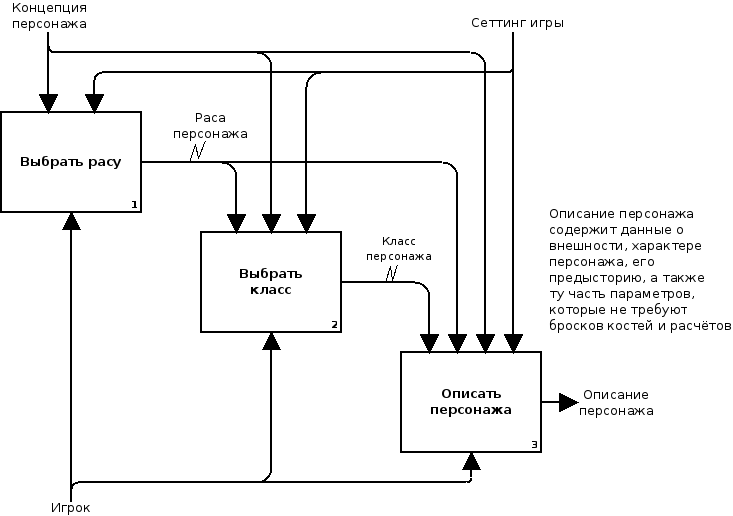
\includegraphics[width=1\linewidth]{images/current_idef/A12.png}}
\caption{Диаграмма A12 исходной информационной системы: описание процесса <<Создать персонажа>>}
\label{ris:current_a12_diagram}
\end{figure}

\begin{figure}[h]
\center{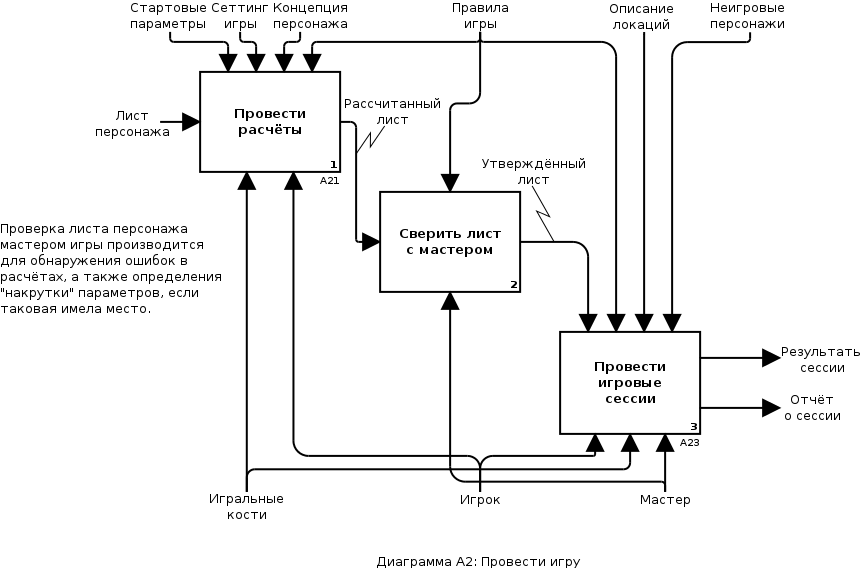
\includegraphics[width=1\linewidth]{images/current_idef/A2.png}}
\caption{Диаграмма A2 исходной информационной системы: описание процесса <<Провести игру>>}
\label{ris:current_a2_diagram}
\end{figure}

\begin{figure}[h]
\center{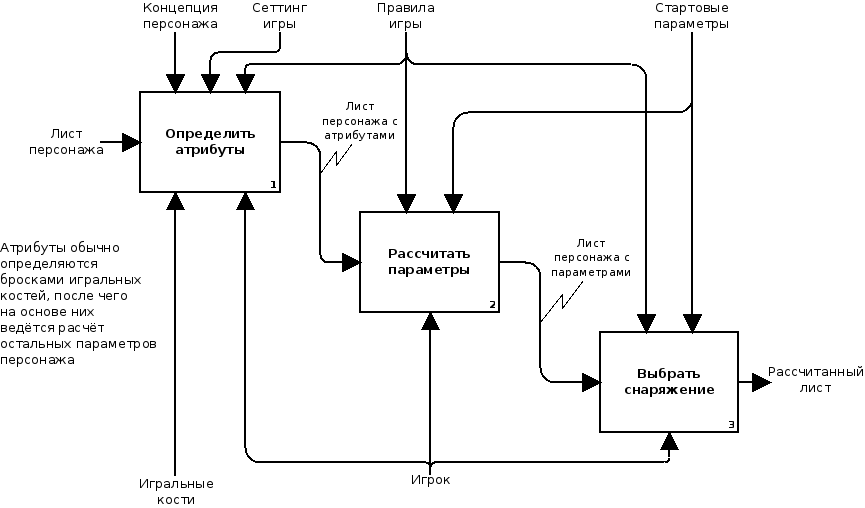
\includegraphics[width=1\linewidth]{images/current_idef/A21.png}}
\caption{Диаграмма A21 исходной информационной системы: описание процесса <<Провести расчёты>>}
\label{ris:current_a21_diagram}
\end{figure}

\begin{landscape}
  \vspace*{\fill}
  \begin{figure}[h]
  \center{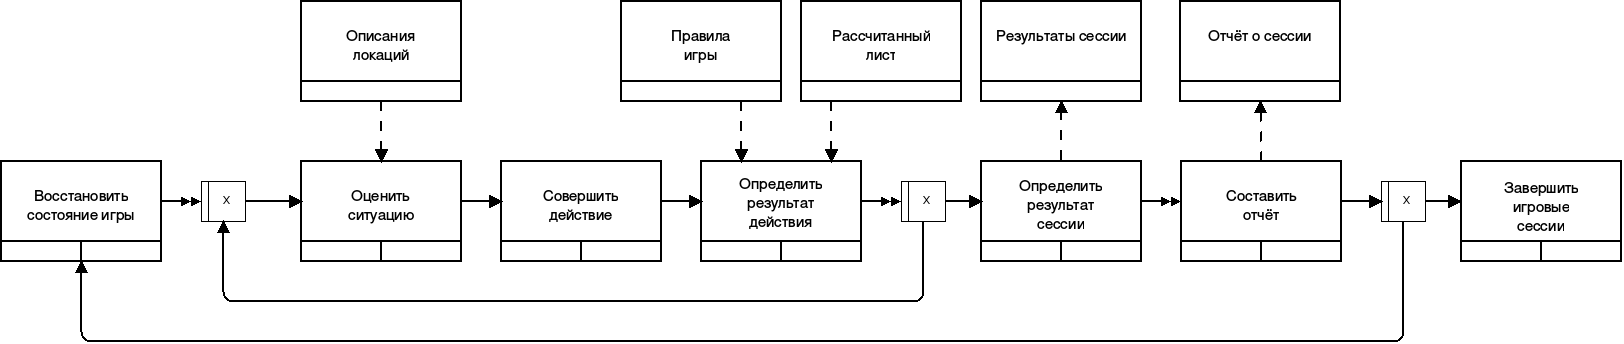
\includegraphics[width=1\linewidth]{images/current_idef/A22.png}}
  \caption{Диаграмма A22 исходной информационной системы: описание процесса <<Провести игровые сессии>>}
  \label{ris:current_a22_diagram}
  \end{figure}
  
\end{landscape}

\begin{figure}[h]
\center{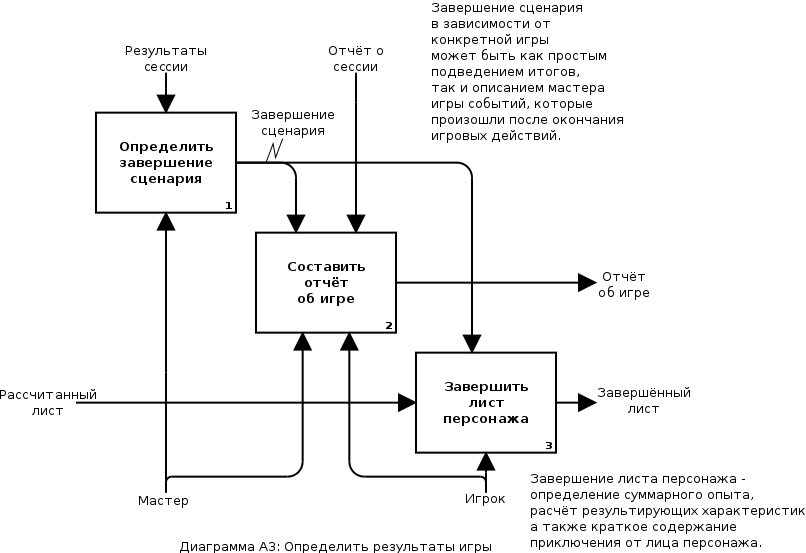
\includegraphics[width=1\linewidth]{images/current_idef/A3.png}}
\caption{Диаграмма A3 исходной информационной системы: описание процесса <<Определить результаты игры>>}
\label{ris:current_a21_diagram}
\end{figure}


Основными недостатками существующей информационной системы являются:
\begin{enumerate}
\item Отсутствие автоматизации расчётов\\
Игровой процесс с использованием ролевой системы \dnd\ включает в себя большое количество расчётов. Исходная модель не предоставляет специализированных средств для их автоматизации, что приводит к большим затратам времени --- от 30\% до 60\% времени обычно занимают расчёты.
\item Отсутствие специализированного средства обмена информацией\\
Для игры с использованием \dnd\ необходим обмен информацией --- как во время игровой сессии так и между сессиями. Обычно этот обмен осуществляется с помощью средств связи или сторонних информационных ресурсов (в т.ч. социальных сетей). Такие способы неэффективны, так как они не позволяют в удобном формате обмениваться специфичной информцией, такой как листы персонажей.
\item Отсутствие централизованного средства хранения информации\\
\dnd\ является набором правил и описаний. Обычно распространение информации происходит с помощью бумажных носителей --- книг и журналов. Количество книг, используемых для игры может быть значительным, а поиск информации в них может занимать длительное время.
\end{enumerate}
